\section{项目实施}
\subsection{实施方案设计}
\subsubsection{实施步骤}
项目按“数据—模型—决策—系统—评估”五个阶段推进，每个阶段都设置可检验的产出，前一阶段验收后再进入下一阶段。

\begin{table}[H]\centering\small
\caption{实施步骤与阶段产出}\label{tab:plan}
\begin{tabularx}{\linewidth}{@{}p{.15\linewidth}XX@{}}\toprule
阶段 & 主要工作 & 验收产出\\\midrule
数据准备 & 选点、调用接口、保存原始响应、质量检查 & 三地原始JSON与哈希清单，缺失与范围检查记录\\
模型构建 & 特征工程、时间划分、模型训练、共形校准 & 已训练模型、特征列表、校准分位数\\
决策规则 & 作物系数情景、水量平衡与供水约束实现 & 规则函数与独立公式核验测试\\
系统开发 & 推理接口、交互界面、记录导出 & 本地可运行的决策工作台\\
评估与诊断 & 时间留出测试、迁移检验、180组仿真 & 逐日预测、仿真明细、诊断图表与本报告\\\bottomrule
\end{tabularx}
\end{table}

\subsubsection{资源配置}
项目全部基于开源工具与公开数据完成。软件环境为Python 3.12及NumPy、pandas、scikit-learn、Matplotlib等库，界面使用浏览器原生HTML、CSS与JavaScript；硬件为普通笔记本电脑，训练与推理均在CPU上完成，无需GPU或云服务。数据为Open-Meteo提供的ERA5再分析逐日气象，按CC BY 4.0许可使用\cite{license}。

\subsubsection{团队分工}
团队成员按工作包分工协作，每个工作包设负责人，交叉审阅彼此的代码与结果。

\begin{table}[H]\centering\small
\caption{工作包与职责}\label{tab:team}
\begin{tabularx}{\linewidth}{@{}p{.20\linewidth}X@{}}\toprule
工作包 & 职责\\\midrule
数据与模型 & 数据获取与质量控制、特征工程、模型训练与共形校准、对照与迁移实验\\
决策与仿真 & FAO-56水量平衡规则、灌溉策略设计、180组情景仿真与敏感性分析\\
系统与材料 & 推理服务与交互界面开发、测试、技术方案、答辩材料与演示视频\\\bottomrule
\end{tabularx}
\end{table}

\subsection{关键技术实现}
\subsubsection{从参考蒸散到作物需水}
预测层输出参考蒸散$\widehat{\mathrm{ET}}_0$，决策层乘以作物系数得到当日需水估计：
\begin{equation}\label{eq:crop}
\widehat E_t=K_{c,t}\,\widetilde{\mathrm{ET}}_{0,t},
\end{equation}
其中点预测策略取$\widetilde{\mathrm{ET}}_{0,t}=\widehat{\mathrm{ET}}_{0,t}$，上界策略取$\widetilde{\mathrm{ET}}_{0,t}=\widehat{\mathrm{ET}}_{0,t}+q$。仿真以5—9月为示范生长季，参照FAO-56玉米分阶段作物系数的变化形态，月度$K_c$依次设为0.45、0.80、1.15、1.15和0.70（实际应用时按当地播期与生育期调整）。表\ref{tab:assumptions}汇总仿真参数。

\begin{table}[H]\centering\small
\caption{灌溉仿真参数}\label{tab:assumptions}
\begin{tabularx}{\linewidth}{@{}l l X@{}}\toprule
参数 & 取值 & 说明\\\midrule
生长季 & 5—9月 & 示范生长季，共153天\\
TAW & 80/120/160 mm & 三档土壤总可用水，覆盖轻质到中壤质土壤在常见根深下的范围\\
灌溉效率$\eta$ & 0.70/0.85 & 分别代表较低与较高的灌溉水利用水平\\
易利用水比例$p$ & 0.50 & 触发阈值$\mathrm{RAW}=p\,\mathrm{TAW}$\\
回填目标比例$\beta$ & 0.25 & 灌溉后目标亏缺占TAW的比例\\
初始亏缺 & $0.35\,\mathrm{TAW}$ & 各策略同一起点\\
有效降水比例$\rho$ & 0.80 & 降水折算为有效补给\\
日毛灌溉上限$C$ & 40 mm & 仿真统一上限，界面可调\\\bottomrule
\end{tabularx}
\end{table}

\subsubsection{触发与回填规则}
令$D_t$为当天决策前的根区亏缺，$0\le D_t\le\mathrm{TAW}$，$D_t=0$表示根区处于田间持水状态，$D_t=\mathrm{TAW}$表示可用水耗尽，界面中的“剩余可用水”即$\mathrm{TAW}-D_t$。决策时尚不知道当天降水，因此预计亏缺为
\begin{equation}\label{eq:projected}
D_t^*=D_t+\widehat E_t.
\end{equation}
未考虑供水上限时的毛灌溉需求为
\begin{equation}\label{eq:requirement}
I_t^{\rm req}=\begin{cases}
0,&D_t^*\le p\,\mathrm{TAW},\\[2pt]
\dfrac{D_t^*-\beta\,\mathrm{TAW}}{\eta},&D_t^*>p\,\mathrm{TAW}.
\end{cases}
\end{equation}
考虑供水能力后，实际毛灌溉量和净补水量为
\begin{equation}\label{eq:capacity}
I_t=\min\{C,I_t^{\rm req}\},\qquad I_t^{\rm net}=\eta I_t.
\end{equation}
“毛灌溉”是输入田间的等效水深，“净补水”是扣除损失后进入根区的水量；效率越低，补足同样亏缺所需的毛用水越多。若$I_t^{\rm req}>C$，服务端标记供水受限，并给出补水后的预计亏缺$D_t^*-\eta I_t$，提示使用者安排后续补灌。

以$\mathrm{TAW}=120$ mm、$K_c\widetilde{\mathrm{ET}}_0=5$ mm为例：$D_t=55$ mm时$D_t^*=60$ mm，恰等于阈值，不灌溉；$D_t=56$ mm时触发灌溉，毛灌溉量为$(61-30)/0.85=36.5$ mm。阈值附近的微小差异会使动作从“不灌”跳到“回填”，这正是需水预测精度与不确定性对灌溉决策产生实际影响的地方。

\subsubsection{日末水量平衡}
仿真在决策后读取当天实际降水$P_t$与参考蒸散$\mathrm{ET}_{0,t}$，令$E_t=K_{c,t}\mathrm{ET}_{0,t}$，未截断的日末亏缺为
\begin{equation}\label{eq:balance}
B_t=D_t+E_t-\rho P_t-\eta I_t,
\end{equation}
并分解为
\begin{align}
D_{t+1}&=\clip(B_t,0,\mathrm{TAW}),\label{eq:clip}\\
Q_t&=\max(0,-B_t),\label{eq:drain}\\
\mathcal U_t&=\max(0,B_t-\mathrm{TAW}),\label{eq:unmet}
\end{align}
其中$Q_t$为超过根区储水上限的排水，$\mathcal U_t$为可用水耗尽后无法满足的需水，满足守恒关系$B_t=D_{t+1}+\mathcal U_t-Q_t$，用于逐日一致性检查。季节评价量为
\begin{align}
W&=\sum_t I_t,&S&=\sum_t\mathbf 1(D_{t+1}>\mathrm{RAW}),\\
Q&=\sum_t Q_t,&\mathcal U&=\sum_t \mathcal U_t,
\end{align}
分别为季节毛灌溉量、缺水风险日、排水量和未满足需水量。

\subsubsection{五种灌溉策略}
\begin{itemize}
\item \textbf{定额日历}：从生长季首日起每7天灌25 mm，代表按固定周期灌溉的传统做法；
\item \textbf{墒情阈值}：只看当前亏缺，$D_t>0.5\,\mathrm{TAW}$时回填至$0.25\,\mathrm{TAW}$，代表有墒情监测但不做预测的做法；
\item \textbf{昨日值预测}：式\eqref{eq:requirement}中以昨日ET\textsubscript{0}作为次日预测；
\item \textbf{AI点预测}：以梯度提升树点预测代入；
\item \textbf{AI区间上界}：以点预测加校准分位数$q$代入，偏向降低缺水风险。
\end{itemize}
每个“地区×年份×TAW×效率”组合构成一个环境情景：
\begin{equation}
3\text{地}\times2\text{年}\times3\text{档TAW}\times2\text{档效率}=36\text{个情景},
\end{equation}
五种策略共180组季节轨迹，每组153天，合计27540条逐日记录。所有策略共享同一气象序列、初始亏缺与作物系数，且在决策时都不知道当天降水，保证比较公平。

\subsubsection{推理服务与接口}
数据处理、模型训练与仿真位于\file{src/pipeline.py}，水量公式与参数校验位于\file{src/agro.py}。服务启动时加载模型、特征列表、校准分位数与逐日结果，提供三个接口（表\ref{tab:api}）。

\begin{table}[H]\centering\small
\caption{本地服务接口}\label{tab:api}
\begin{tabularx}{\linewidth}{@{}p{.30\linewidth}XX@{}}\toprule
接口 & 作用 & 关键约束\\\midrule
\texttt{GET /api/summary} & 读取实验概要 & 与报告数据同源\\
\texttt{GET /api/forecast} & 目标日推理与历史曲线 & 地区与日期在服务端校验\\
\texttt{POST /api/recommend} & 计算灌溉建议 & 服务端重新推理，参数逐项校验\\\bottomrule
\end{tabularx}
\end{table}

建议接口不接受页面提交的预测值，而是根据地区和日期在服务端重新调用模型，防止被篡改的浏览器状态冒充模型输出。参数必须为有限数值：TAW为40\,$\sim$\,240 mm，效率为0.4\,$\sim$\,1，供水上限为0\,$\sim$\,100 mm，作物系数为0.1\,$\sim$\,1.5，亏缺不得超过TAW。前端为每次请求编号并与当前输入签名比对，快速连续修改参数时，较晚返回的旧结果不会覆盖新状态。导出记录包含地区、日期、策略、全部输入、点预测与上界、模型训练截止日和校准截止日。

\subsubsection{交互界面}
界面分为“需水与灌溉”“模型验证”“策略回测”三个视图（图\ref{fig:ui}）。首屏并列显示预测ET\textsubscript{0}、90\%区间、昨日值基线和事后参考值；曲线图以阴影表示预测区间，可悬停查看逐日数值并切换30日、90日窗口；根区水量条以同一毫米标尺显示剩余可用水、当前亏缺与触发线；右侧参数面板实时给出建议量与依据。视觉上采用低饱和灰绿与米白配色，突出数值与对比关系。

\begin{figure}[H]\centering
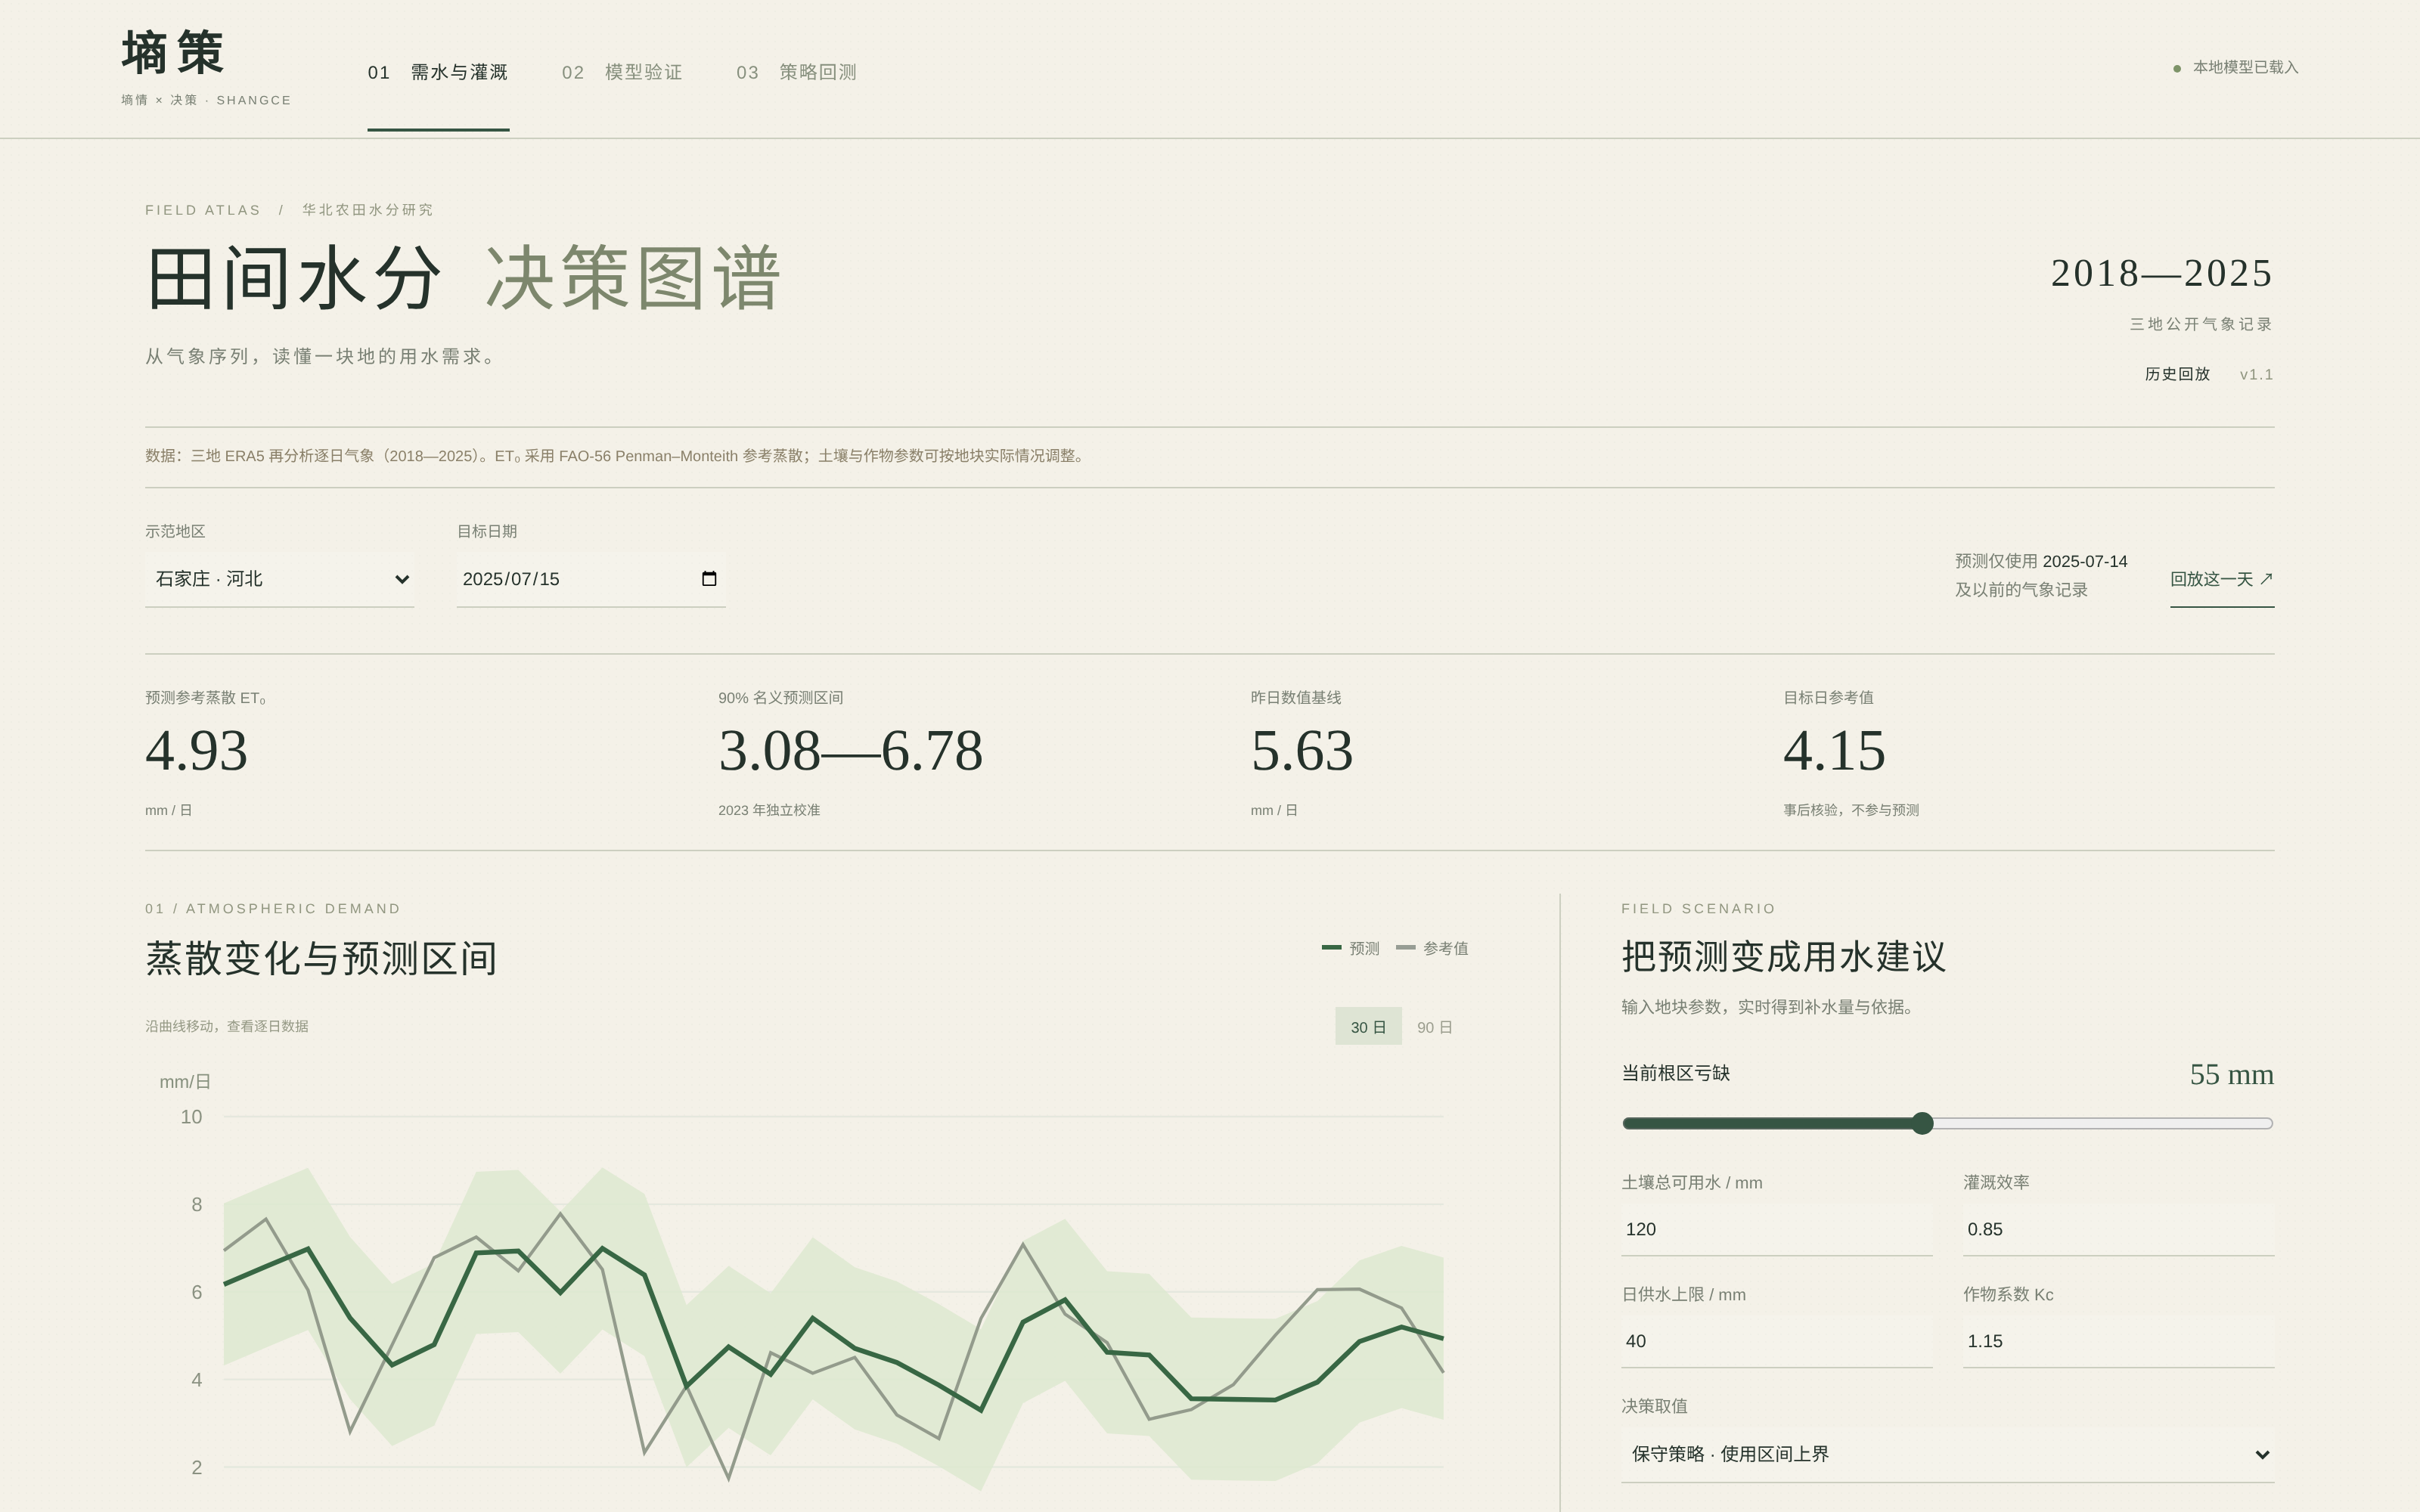
\includegraphics[width=.92\linewidth]{../results/screenshots/dashboard.png}
\caption{“需水与灌溉”视图：次日需水预测、预测区间与灌溉建议}\label{fig:ui}
\end{figure}

图\ref{fig:capacity}演示供水能力受限的情形：将日供水上限设为5 mm后，系统按上限给出5 mm毛灌溉量，提示供水能力不足，并显示补水后的预计亏缺。

\begin{figure}[H]\centering
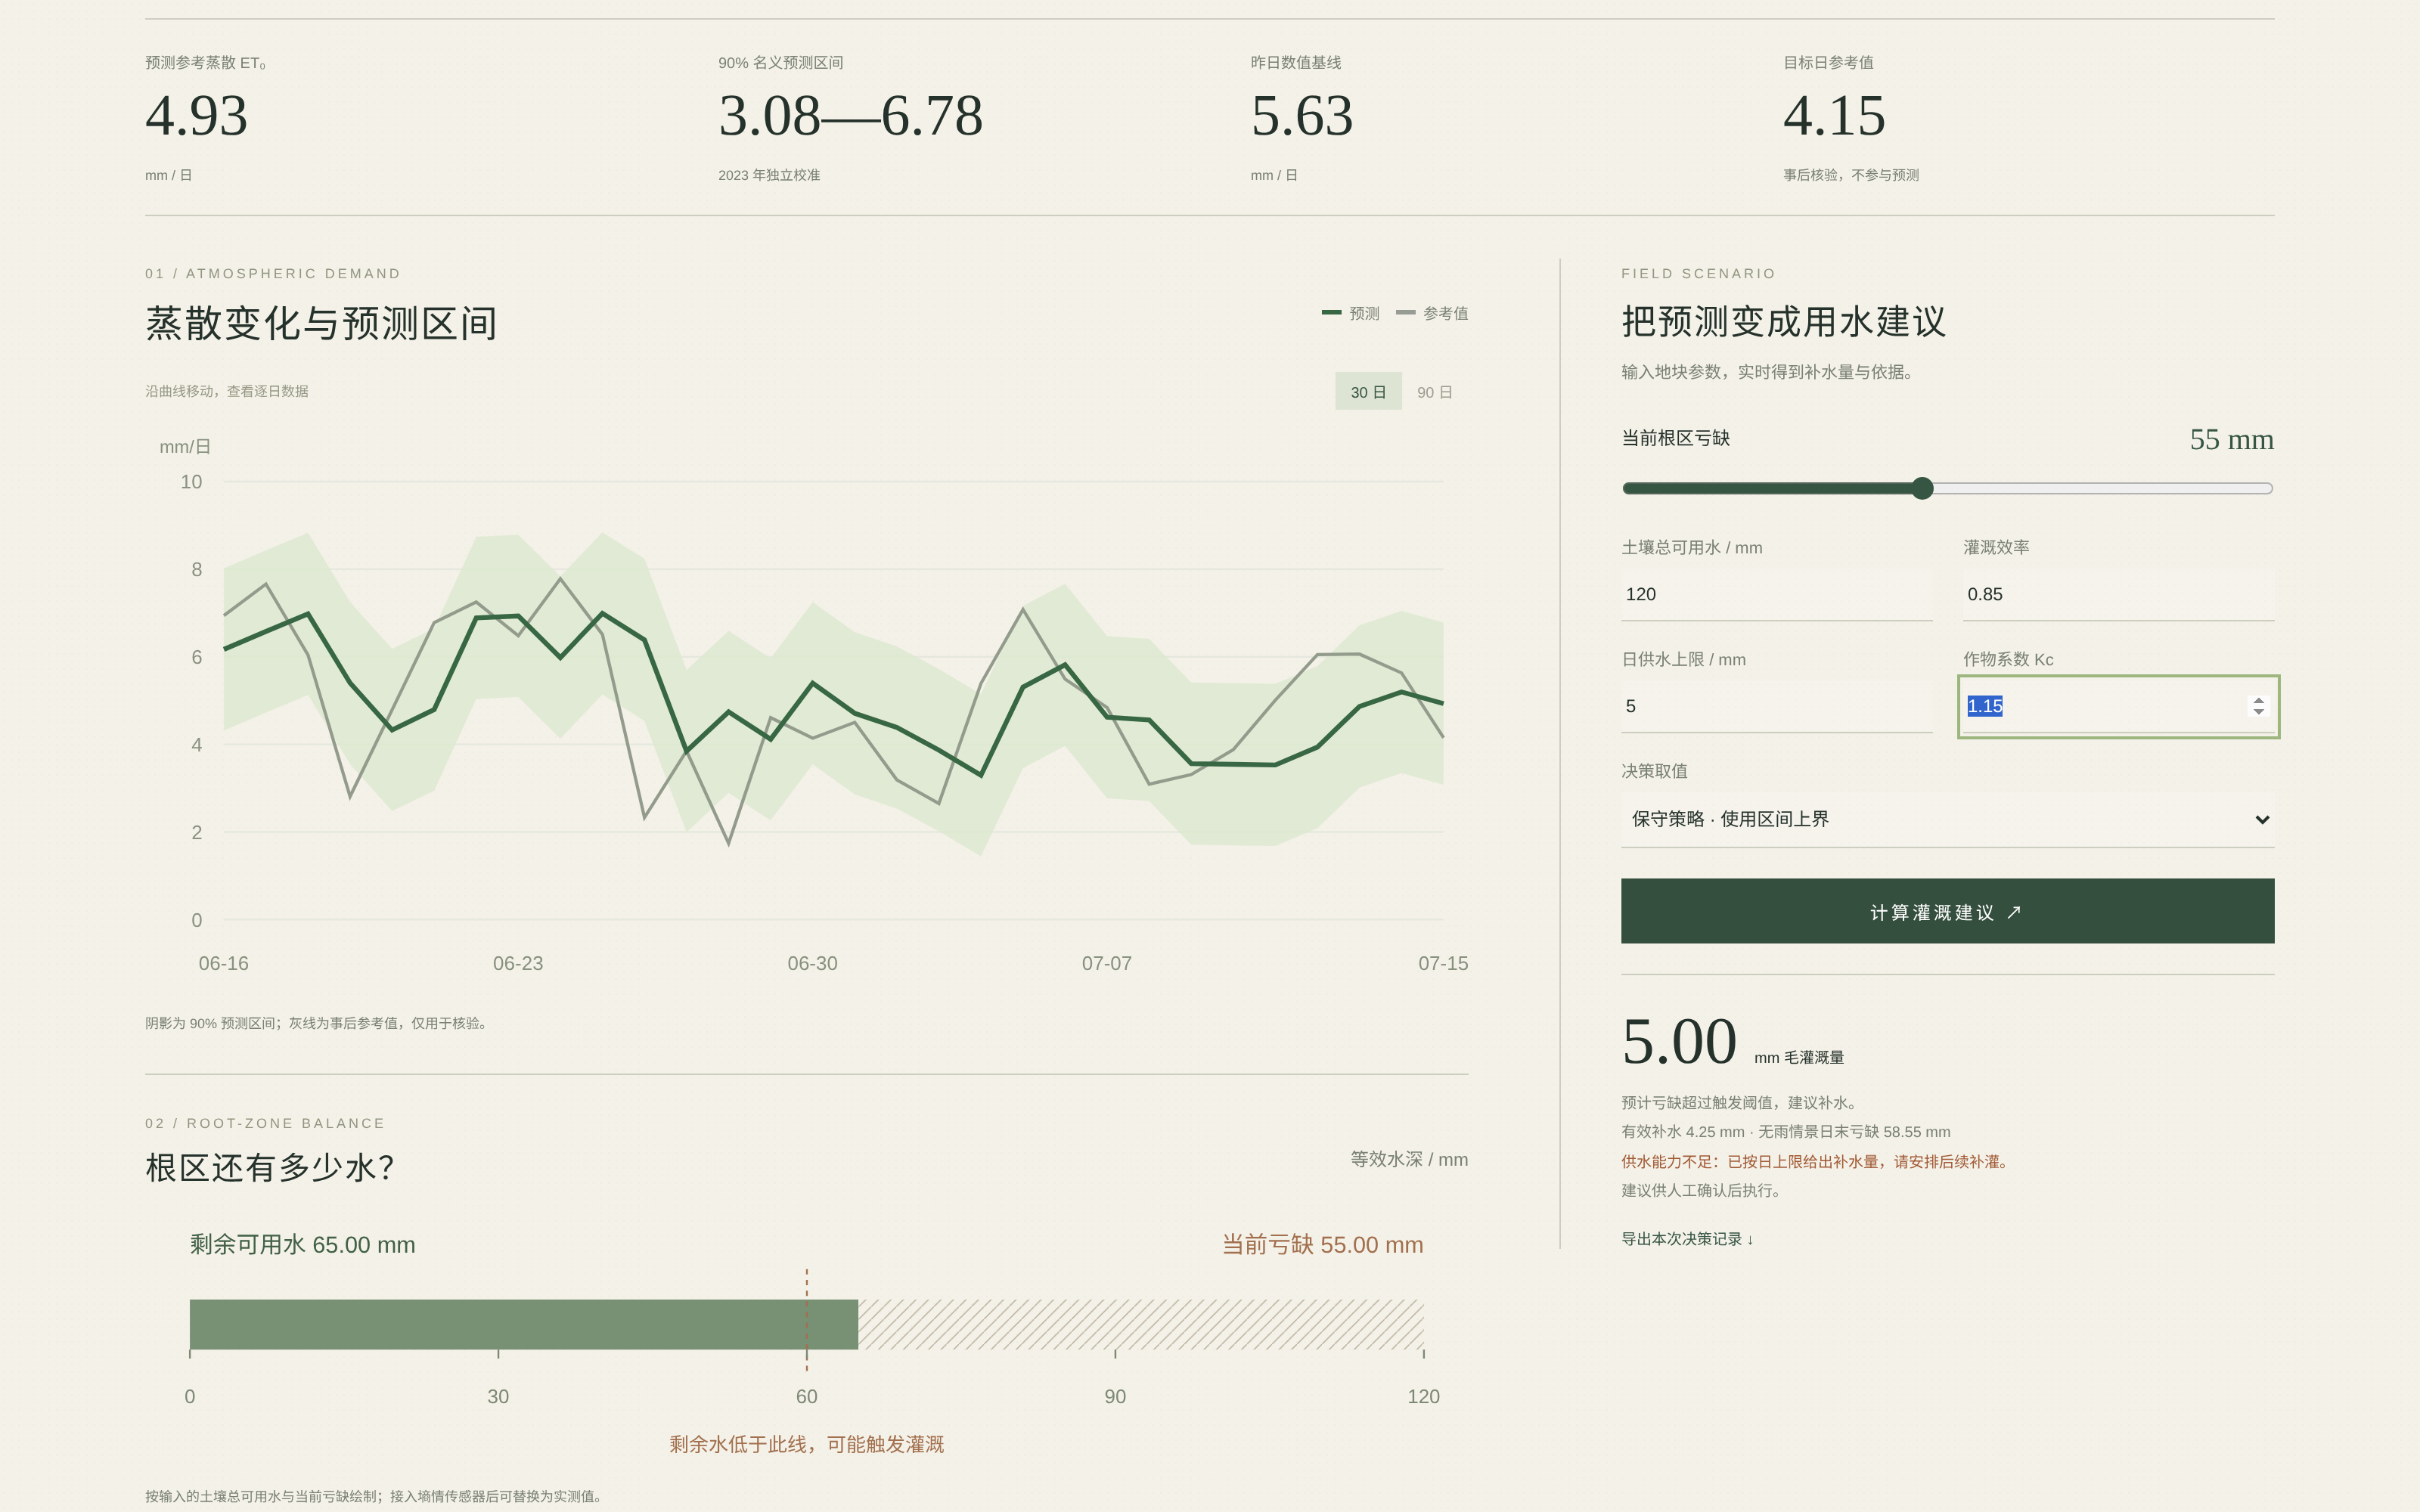
\includegraphics[width=.92\linewidth]{../results/screenshots/capacity.png}
\caption{供水上限为5 mm时的建议结果与能力不足提示}\label{fig:capacity}
\end{figure}

\subsubsection{测试与质量保障}
\begin{itemize}
\item \textbf{核心测试（9项，全部通过）}：未来数据扰动不改变特征、区间分位数计算、水量守恒、阈值边界、供水上限、非有限数值拒绝等；
\item \textbf{浏览器测试（9项，全部通过）}：初始推理、能力不足提示、JSON导出与页面输入一致、模型表与策略表渲染、非法输入禁止导出及恢复、手机布局无横向溢出、无未捕获异常；
\item \textbf{交付核验（61项，全部通过）}：从CSV重算MAE、RMSE、$R^2$与覆盖率，逐日水量汇总与180组季节结果一致，原始输入哈希匹配。
\end{itemize}
